\section{Introduction}\label{sec:introduction}
Ancient mariners could look up the night sky, point out what stars they were looking at, and navigate across the globe
with precision. \textit{Star identification algorithm} refers to a computational approach to pointing out which stars
are in the sky. Given an image of the sky, star identification is matching the bright spots in an image, to stars in an
astronomical catalog. The device that performs these computations is the star tracker, much like the navigators on the
ship. \textit{Lost-in-space} refers to an additional constraint on the problem: the absence of knowing where we took
the picture and how we pointed the camera.

This problem is most prevalent in designing LEO (low Earth orbit) spacecraft. In order for a craft to point a payload,
direct thrusters, or orient it's solar panels, an accurate \textit{attitude} (another term for orientation) must be
known. There are a few known landmarks in space where some attitude can be extracted (the Earth, the Sun), but this
requires constant direction towards just these objects. Star trackers do not limit themselves to a single object,
rather they use the entire sky of stars to determine it's orientation.

This paper analyzes six existing identification methods, all of which involve the following process:
\begin{enumerate}
    \item Given an image of stars.
    \item Identify a select few stars in the image.
    \item Guess how we are oriented.
    \item Identify the rest of the stars in the image.
    \item Finalize and determine our orientation.
\end{enumerate}

Each method's feature uniqueness, permutation order, candidate reduction, and alignment determination will be
characterized under the introduction of various noise. The process of identifying blobs in an image, constructing
the image coordinate system, and efficiently querying static databases is not addressed here.

There has been an increasing number of approaches toward stellar attitude determination, but little comparison between
each of these methods in a more controlled manner. Interchangeable factors are abstracted away (camera hardware, blob
detection, etc\ldots) to focus more on how each method matches stars in an image to a catalog.

\section{Attitude Determination}\label{sec:attitudeDetermination}
Attitude determination is the process of finding one's orientation in space. On Earth, "up" and "down" mean "up from
the center of the Earth" and "down toward the center of the Earth". The direction toward the Earth can be determined
using the Earth's gravitational presence. This makes attitude determination fairly straightforward, requiring no more
than a 3-axis acceleration sensor. These are present inside most(if not all) modern cell phones.

In space, distinguishing "up from Earth" from "down toward Earth" is different as the Earth's gravitational presence is
severely diminished. This means that the acceleration sensors used here cannot be used to determine one's attitude in
space. Spacecraft instead use other objects to build an attitude from. The visual position of the Sun and the Earth's
magnetic field are common choices for reference points, but the most popular are the visual positions of various stars
in the sky.

% https://commons.wikimedia.org/wiki/File:Moving_coordinate_system.PNG
\begin{figure}
    \centering{
    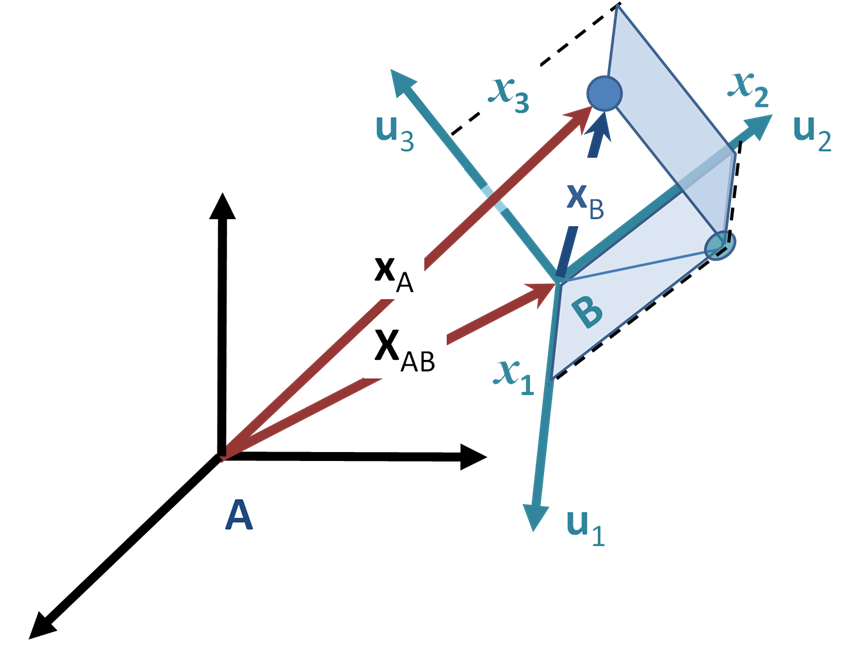
\includegraphics[scale=0.23]{images/moving-coordinate-systems.PNG}
    \caption{
    Visual of two coordinate frames: the inertial frame $A$, and the body frame $B$ from (citation here). The point $x$
    is observed with vector $x_A$ in the $A$ frame, but the same point $x$ is observed with vector $x_B$ in the $B$
    frame. By aligning several observations in both frames, a spacecraft orientation $x_{AB}$ in the $B$ frame can be
    determined in the $A$ frame.
    } \label{figure:coordinateSystem}
    }
\end{figure}

Once some known object is found by the sensor, these measurements exists in a \textit{body reference frame}. This
reference frame reveals the position of objects with respect to the sensor, but is not fixed to any point. There exists
a separate, fixed frame with which these known objects are recorded in prior to the start of the mission. This is known
as an \textit{inertial reference frame}.~\autoref{figure:coordinateSystem} depicts the relation between both
frames. Given sensor measurements to a set of points ($X_A, X'_A, X''_A, \ldots$) and inertial frame
measurements to the same objects ($X_B, X'_B, X''_B, \ldots$), the goal of attitude determination involves
finding the rotation $X_{AB}$ to take all points in the sensor frame to the inertial frame (or the inverse). In
short, attitude determination involves taking inertial frame object observations in the body frame, and figuring out
how the spacecraft is oriented in this inertial frame.

From here, the problem becomes aligning vector observations in the body frame with another set of vectors in the
inertial frame. This is known as \textit{Wahba's problem}, and is a form of an optimization problem. A popular and
simple method to extract an attitude from two vectors in both the inertial and body frame is the \textit{TRIAD method}.
For all instances where Wahba's problem was present, the TRIAD method was used to extract an orientation.

\subsection{Stellar Based Attitude Determination}\label{subsec:stellarBasedAttitudeDetermination}
Relative to our solar system, the majority of bright stars ($m < 6.0$, or visible from the Earth without a telescope)
\textit{do not visibly move}. Most of these stars exist hundreds of lightyears away from the solar system. Observing a
tiny change in a star's position from Earth suggests a massive change in position relative to the star. For many LEO
missions, the time it takes for these star positions to change is longer than the length of mission itself. For longer
missions, only then will star dynamics have to be taken into account. This paper address spacecraft missions where all
stars are virtually static in position.

A basic star tracker is composed of a camera, a computer for determining orientation, and a link back to the main
computer. Once the star tracker on a lost-in-space spacecraft takes a picture, three main pieces of information are
known:
\begin{enumerate}
    \item An 2D image of the sky.
    \item Characteristics of the camera hardware (field-of-view, lens structure, \ldots).
    \item All cataloged stars and their 3D positions in the catalog (inertial) frame.
\end{enumerate}

After taking the picture, the pixel positions of stars in the image are determined. This involves finding bright blobs
in the image, and finding each blob's center of mass. To align these stars with the ones in the catalog, the image must
be projected into 3D. This is done using the items in (2) above, and can be a major source of error if these
characteristics are not accurate. The result of this process are star vectors in the image (body) frame.

By running these image star vectors through a star identification method, an \textit{alignment} between the image frame
stars and catalog frame stars is found. For a given image star $b$ and a catalog star $r$, an alignment $a$ describes
an association ($b, r$) between both stars. This then reduces to Wahba's problem, and is solved using the TRIAD method
to obtain a spacecraft attitude.